\FloatBarrier
\section{Connectivity, Parallel Gates and Spectator Response}
\label{app:array-parallel-control}
\label{chap:quantum-processors}

Section~\ref{sec:platform-array-selection} states the conditions for
selecting spins and exchange links. This appendix derives the spectator
response and the restrictions on scheduling independent gates.

The available exchange links specify which physical spins can interact
directly. Several selected links may share a spin, and a control field
may also reach a spin outside the selected set. This appendix examines
how physical connectivity, encoded blocks and unwanted couplings
constrain operations on an array. Its parallel-gate and spectator
calculations give conditions for the intended operations to act
independently during a shared interval.

\subsection{Connectivity and layout}
\label{sec:connectivity-layout}

An exchange gate between electron spins requires tunneling between
their dots. The positions of the dots therefore restrict which
pairs can interact directly. Represent each dot by a vertex and
each controllable exchange coupling by an edge. For a single-spin
array, a useful model is
\begin{equation}
 H(t)=\sum_i E_{Z,i}(t)s_{iz}
       +\sum_{(i,j)\in\mathcal E}J_{ij}(t)
                   \mathbf s_i\cdot\mathbf s_j
       +H_{\mathrm{drive}}(t),
 \label{eq:processor-array-hamiltonian}
\end{equation}
where \(\mathcal E\) is the set of available exchange links,
\(\mathbf s_i=\boldsymbol{\sigma}_i/2\), and
\(H_{\mathrm{drive}}\) contains transverse spin controls. An edge
states that \(J_{ij}\) can be made useful for a gate; it does not
assert that this coupling is always on. Conversely, a pair without
an edge has no direct exchange gate in this model.

Consider the four-dot chain in
Fig.~\ref{fig:processor-four-dot-exchange}, with
\(\mathcal E=\{(1,2),(2,3),(3,4)\}\). To act only on spins 2 and 3,
we raise \(J_{23}\) while keeping the other two couplings small.
If \(J_{12}\) is also appreciable, spin 2 interacts with both
neighbours and the pulse is a three-spin operation. For a residual
coupling approximately constant over a duration \(\tau\), the
unwanted exchange area is \(J_{\mathrm{off}}\tau/\hbar\). It is this
area, rather than a binary on/off description, that sets the scale
of its possible effect. The on-setting must also keep the selected
spins in their intended computational space, as established for
the individual gate constructions in
Appendices~\ref{app:single-spin-control}, \ref{app:st-control}
and~\ref{app:exchange-only-control}.


A physical dot and an encoded qubit need not be the same object.
The basic operating blocks considered here have
\begin{center}
\begin{tabular}{lcc}
\hline
Encoding & Dots per qubit & Dots in a two-qubit block\\
\hline
Single spin & 1 & 2\\
Singlet--triplet & 2 & 4\\
Exchange only & 3 & 6\\
\hline
\end{tabular}
\end{center}
These counts assume one electron per dot during the spin operation
and omit reservoirs, sensors and spare dots. A link inside a
three-dot exchange-only block gives a logical one-qubit rotation;
the boundary link in
Fig.~\ref{fig:processor-exchange-only-blocks} is one ingredient
of a six-spin two-qubit sequence, not a complete logical gate. Two
singlet--triplet blocks can instead obtain a conditional phase
from their state-dependent charge distributions, as in
Section~\ref{sec:calibration-controlled-phase}. The graph of
usable \emph{logical} gates is obtained only after each complete
physical sequence has been specified and shown to return to the
logical spaces.

\begin{figure}[htbp]
 \centering
 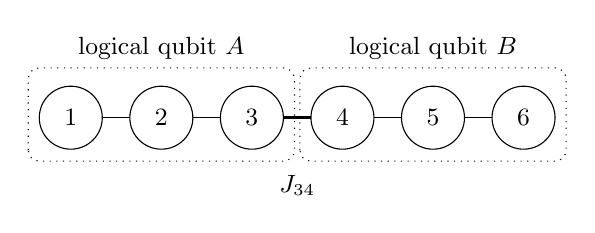
\begin{tikzpicture}[x=1.15cm,y=1.15cm,
   every node/.style={font=\small}]
  \draw[dotted,rounded corners] (-0.47,-0.48) rectangle (2.47,0.55);
  \draw[dotted,rounded corners] (2.53,-0.48) rectangle (5.47,0.55);
  \node at (1,0.77) {logical qubit $A$};
  \node at (4,0.77) {logical qubit $B$};
  \draw[thin] (0,0)--(1,0)--(2,0);
  \draw[very thick] (2,0)--(3,0);
  \draw[thin] (3,0)--(4,0)--(5,0);
  \foreach \x/\lab in {0/1,1/2,2/3,3/4,4/5,5/6} {
   \node[draw,circle,fill=white,minimum size=8mm,inner sep=0pt]
     at (\x,0) {$\lab$};
  }
  \node at (2.5,-0.75) {$J_{34}$};
 \end{tikzpicture}
 \caption{Two exchange-only qubits formed from six physical dots.
 Each dotted box groups the three spins of one logical qubit.
 The thick \(J_{34}\) boundary link is a physical exchange coupling,
 not a complete logical two-qubit gate.}
 \label{fig:processor-exchange-only-blocks}
\end{figure}
\FloatBarrier

The graph also determines the cost of an operation between
non-neighbours. In the four-dot chain of
Fig.~\ref{fig:processor-four-dot-exchange}, there is no
exchange edge
\((1,3)\); pulsing one barrier cannot implement a gate on spins
1 and 3. A circuit must route a state along existing edges,
move an electron, or use another mediator. The number of edges
along a chosen path, not the distance between labels on a drawing,
sets the elementary routing count. A two-dimensional
layout offers different paths, although interior dots also need
control and readout access. A six-dot device may encode six
single-spin qubits or two exchange-only qubits, so dot count alone
does not describe its connectivity or computational capacity.
A six-spin silicon register has demonstrated coordinated
preparation, gates and measurement in one array~\cite{Philips2022}.

\subsection{Parallel gates and spectator response}
\label{sec:addressing-parallel-operation}

A set of gates is independent during one interval only if its
complete evolution has the intended action on both the selected
spins and the spectators. The exchange graph constrains whether
two selected pair gates share a spin. The spatial and frequency
response of the drive determines what happens to spins outside
the selected set. These are distinct restrictions on parallel
operation.

\subsubsection{Independent exchange gates on a graph}
\label{sec:processor-parallel-exchange}

Consider four occupied dots in a chain. Raising exchange on
\((1,2)\) and \((3,4)\) couples disjoint spin pairs. Their
Hamiltonians act on different tensor factors, so the two
pair operations can run during the same interval in the ideal
model. Raising exchange on \((1,2)\) and \((2,3)\) has a
different meaning: spin 2 interacts with both neighbours.
With \(H_{ij}=J_{ij}\mathbf s_i\cdot\mathbf s_j\),
\[
 [H_{12},H_{34}]=0,\qquad [H_{12},H_{23}]\ne0.
\]
For constant simultaneous couplings on the adjacent edges,
the evolution is
\[
 U_{\mathrm{sim}}
 =e^{-i(H_{12}+H_{23})\tau/\hbar}.
\]
It is a three-spin operation, not the product of two
independently calibrated pair gates. The same distinction
holds for shaped pulses: the shared spin still belongs to
both Hamiltonian terms at once. Such a pulse can be useful
if its complete three-spin action is designed, but it
cannot simply replace two successive pair gates.

For isolated pair gates, a set of edges with no shared
vertex is therefore one candidate layer. Figure~
\ref{fig:processor-gate-layers} shows two such layers on a
six-spin chain. The first uses \((1,2),(3,4),(5,6)\);
the second uses \((2,3),(4,5)\). Together they cover
the nearest-neighbour edges while assigning each spin
to at most one gate in each interval.

\begin{figure}[htbp]
 \centering
 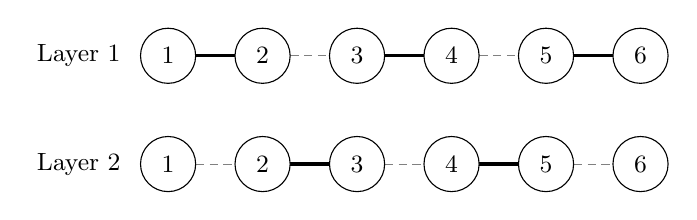
\begin{tikzpicture}[x=1.2cm,y=1.1cm,
   every node/.style={font=\small}]
  \node[anchor=east] at (-0.4,1.25) {Layer 1};
  \node[anchor=east] at (-0.4,0) {Layer 2};
  \draw[very thick] (0,1.25)--(1,1.25);
  \draw[densely dashed,gray] (1,1.25)--(2,1.25);
  \draw[very thick] (2,1.25)--(3,1.25);
  \draw[densely dashed,gray] (3,1.25)--(4,1.25);
  \draw[very thick] (4,1.25)--(5,1.25);
  \draw[densely dashed,gray] (0,0)--(1,0);
  \draw[very thick] (1,0)--(2,0);
  \draw[densely dashed,gray] (2,0)--(3,0);
  \draw[very thick] (3,0)--(4,0);
  \draw[densely dashed,gray] (4,0)--(5,0);
  \foreach \x/\lab in {0/1,1/2,2/3,3/4,4/5,5/6} {
   \node[draw,circle,fill=white,minimum size=7mm,inner sep=0pt]
     at (\x,1.25) {$\lab$};
   \node[draw,circle,fill=white,minimum size=7mm,inner sep=0pt]
     at (\x,0) {$\lab$};
  }
 \end{tikzpicture}
 \caption{Two layers of pair-exchange gates on a six-spin chain.
 Thick edges are scheduled gates; dashed edges are not selected
 for that layer. Residual exchange on an unselected edge must
 still be included in the calibrated operation.}
 \label{fig:processor-gate-layers}
\end{figure}
\FloatBarrier

The dashed links in the figure are unselected, not
mathematically absent. If they retain exchange during a
layer, their accumulated coupling changes its operation.
The graph rule tells us which pair gates do not compete
for the same spin; it does not establish that the voltage
waveform actually suppresses every other coupling.

\subsubsection{Response of spins outside the scheduled gates}
\label{sec:processor-spectator-addressing}

A control pulse can extend beyond the vertex or edge it
was meant to address. For example, a microwave field
resonant with spin \(i\) can also reach a neighbouring
spin \(j\). The latter sees both a transverse drive and
a frequency mismatch. In the frame rotating with the
drive at \(\omega_i\), its Hamiltonian is
\[
 H_j=\frac{\hbar}{2}(-\Delta_j Z_j+\Omega_j X_j),
 \qquad \Delta_j=\omega_j-\omega_i.
\]
Here \(\Omega_j\) is the amplitude at \(j\), not the
programmed amplitude at \(i\). Figure~
\ref{fig:processor-spectator-axis} shows the carrier
frequency relative to the two spin resonances and the
spectator's effective rotation axis. When that axis is
nearly longitudinal, a \(Z_j\) eigenstate barely flips;
a superposition can nevertheless change phase.

\begin{figure}[htbp]
 \centering
 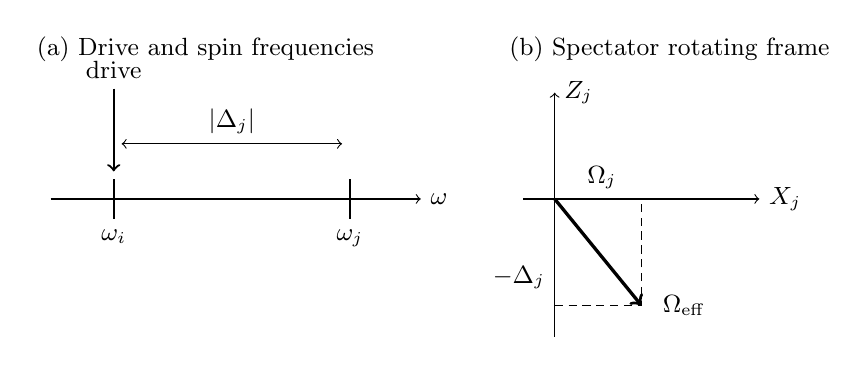
\begin{tikzpicture}[x=1cm,y=1cm,
   every node/.style={font=\small}]
  \node[anchor=west] at (0,2.2) {(a) Drive and spin frequencies};
  \draw[->] (0.3,0.3)--(5.0,0.3) node[right] {$\omega$};
  \draw[thick] (1.1,0.05)--(1.1,0.55);
  \draw[thick] (4.1,0.05)--(4.1,0.55);
  \node[below] at (1.1,0.03) {$\omega_i$};
  \node[below] at (4.1,0.03) {$\omega_j$};
  \draw[->,thick] (1.1,1.7)--(1.1,0.65);
  \node[above] at (1.1,1.7) {drive};
  \draw[<->] (1.2,1.0)--(4.0,1.0);
  \node[above] at (2.6,1.0) {$|\Delta_j|$};
  \node[anchor=west] at (6.0,2.2) {(b) Spectator rotating frame};
  \draw[->] (6.3,0.3)--(9.3,0.3) node[right] {$X_j$};
  \draw[->] (6.7,-1.45)--(6.7,1.65) node[right] {$Z_j$};
  \draw[densely dashed] (6.7,-1.05)--(7.8,-1.05)--(7.8,0.3);
  \draw[->,very thick] (6.7,0.3)--(7.8,-1.05);
  \node[above] at (7.3,0.3) {$\Omega_j$};
  \node[left] at (6.7,-0.7) {$-\Delta_j$};
  \node[anchor=west] at (7.95,-1.05)
    {$\boldsymbol{\Omega}_{\mathrm{eff}}$};
 \end{tikzpicture}
 \caption{A drive resonant with \(i\) is detuned from spectator
 \(j\). Panel (b) depicts \(\Delta_j>0\): the spectator's
 effective rotation vector has transverse component
 \(\Omega_j\) and longitudinal component \(-\Delta_j\).
 Its transverse fraction controls possible flips; its changed
 length also changes the phase accumulated by a superposition.}
 \label{fig:processor-spectator-axis}
\end{figure}
\FloatBarrier

The magnitude of the effective rotation vector is
\(\Omega_{\mathrm{eff}}=\sqrt{\Delta_j^2+\Omega_j^2}\).
For a rectangular pulse lasting \(\tau\), a spectator
initially in \(\ket0_j\) has flip probability
\begin{equation}
 P_{1,j}(\tau)=
 \frac{\Omega_j^2}{\Omega_j^2+\Delta_j^2}
 \sin^2\!\left(
   \frac{\sqrt{\Omega_j^2+\Delta_j^2}\,\tau}{2}\right)
 \leq\frac{\Omega_j^2}{\Omega_j^2+\Delta_j^2}.
 \label{eq:processor-off-resonant-response}
\end{equation}
The prefactor is the squared transverse fraction of
the axis in Fig.~\ref{fig:processor-spectator-axis}.
When \(|\Delta_j|\gg|\Omega_j|\), this bounds the
population transfer even if the pulse duration changes.
A zero of the sine gives no net flip at that particular
duration, but it is not evidence that the pulse left an
arbitrary spectator state unchanged.

The drive also changes the spectator's rotating-frame
level separation. For \(|\Omega_j/\Delta_j|\ll1\),
\(\Omega_{\mathrm{eff}}-|\Delta_j|
 \simeq\Omega_j^2/(2|\Delta_j|)\).
Relative to an otherwise identical wait, the corresponding
additional evolution is
\begin{equation}
 \delta H_j\simeq-\frac{\hbar\Omega_j^2}{4\Delta_j}Z_j,
 \qquad
 U_{j,\mathrm{extra}}\simeq R_z(-\phi_j),\qquad
 \phi_j=\int\frac{\Omega_j(t)^2}{2\Delta_j}\,dt.
 \label{eq:processor-spectator-phase}
\end{equation}
The integral applies to a slowly switched, far-detuned
envelope whose dressed states are followed. A rectangular
pulse may also leave the transverse response quantified by
Eq.~\eqref{eq:processor-off-resonant-response}. Thus a
spectator superposition can acquire a phase even when a
population test finds few flips.

Increasing the target drive can shorten its gate but also
increases the field reaching \(j\). If the measured
cross-drive ratio is \(\Omega_j=c\Omega_i\) with
\(c\ne0\), a rectangular target \(\pi\) pulse takes
\(\tau_\pi=\pi/|\Omega_i|\). Requiring the spectator-flip
envelope to remain below \(0<q<1\) yields
\begin{equation}
 |\Omega_i|\leq
 \frac{|\Delta_j|}{|c|}\sqrt{\frac{q}{1-q}},
 \qquad
 \tau_\pi\geq
 \frac{\pi|c|}{|\Delta_j|}\sqrt{\frac{1-q}{q}}.
 \label{eq:processor-addressing-speed}
\end{equation}
At that speed the spectator phase is approximately
\(\pi c^2|\Omega_i|/(2|\Delta_j|)\) in magnitude,
so the flip limit does not replace a phase check.
Population readout after the target pulse tests flips;
a Ramsey comparison with and without it reveals the
extra phase.

The two parts of this section impose different conditions
on a proposed layer. Disjoint exchange edges prevent one
spin from participating in two intended pair gates.
Spectral separation and cross-drive determine whether an
unselected spin remains idle during a microwave pulse.
Voltage changes can also shift nearby exchange couplings
and spin gaps; disjoint singlet--triplet blocks may acquire
a capacitive phase during parallel local gates
(Section~\ref{sec:calibration-parallel-st-gates}).
Shared drive and readout channels further constrain which
operations can overlap. A layer is justified as a product
of its intended gates, up to calibrated local phases, only
when the complete joint waveform has the required action
on both targets and spectators.
